\documentclass[11pt]{article}
\usepackage[utf8]{inputenc}
\usepackage[T1]{fontenc}
\usepackage{amsmath}
\usepackage{amssymb}
\usepackage{multicol}
\usepackage{geometry}
\usepackage{tikz}
\usepackage{enumitem}
\usepackage{xcolor}
\usepackage{titlesec}

% Configurações de layout
\geometry{a4paper, left=1cm, right=1cm, top=0.5cm, bottom=1.2cm}
\setlength{\columnseprule}{0.4pt}

% Cores para títulos
\titleformat{\section}{\normalfont\Large\bfseries\color{blue}}{\thesection}{1em}{}
\titleformat{\subsection}{\normalfont\large\bfseries\color{red}}{\thesubsection}{1em}{}

\title{\textcolor{red}{Segundo Trimestre: Matemática
    \\Medidas de Dispersão}}
\author{Professor: Jefferson}
\date{}

\begin{document}

\maketitle
\vspace{-1cm}

%\begin{center}
%\large{Nome: \underline{\hspace{8cm}} \quad Turma: \underline{\hspace{3cm}}}
%\end{center}

\begin{multicols}{2}

\section*{Introdução}
Medidas de dispersão indicam o quanto os dados se espalham em torno da média. Enquanto medidas de tendência central mostram o valor típico, as medidas de dispersão mostram a variabilidade.

\section*{Fórmulas Importantes}

\subsection*{Amplitude}

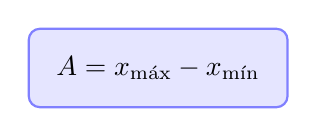
\begin{tikzpicture}
\node[rectangle, fill=blue!10, rounded corners, inner sep=10pt, draw=blue!50, thick] (box) {
$\displaystyle A = x_{\text{máx}} - x_{\text{mín}}$
};
\end{tikzpicture}

\textbf{Onde:}
\begin{itemize}
\item $A$ = amplitude
\item $x_{\text{máx}}$ = maior valor do conjunto
\item $x_{\text{mín}}$ = menor valor do conjunto
\end{itemize}

\subsection*{Variância}

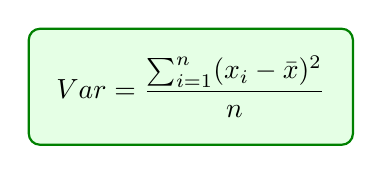
\begin{tikzpicture}
\node[rectangle, fill=green!10, rounded corners, inner sep=10pt, draw=green!50!black, thick] (box) {
$\displaystyle Var = \frac{\sum_{i=1}^n (x_i - \bar{x})^2}{n}$
};
\end{tikzpicture}

\textbf{Fórmula alternativa:}
\[
Var = \frac{\sum x_i^2}{n} - \bar{x}^2
\]

\subsection*{Desvio Padrão}

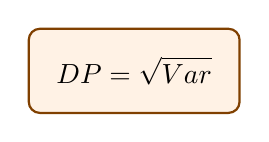
\begin{tikzpicture}
\node[rectangle, fill=orange!10, rounded corners, inner sep=10pt, draw=orange!50!black, thick] (box) {
$\displaystyle DP = \sqrt{Var}$
};
\end{tikzpicture}

\textbf{Unidade:} Mesma unidade dos dados originais

\subsection*{Coeficiente de Variação}

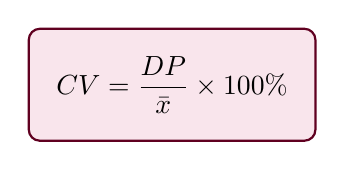
\begin{tikzpicture}
\node[rectangle, fill=purple!10, rounded corners, inner sep=10pt, draw=purple!50!black, thick] (box) {
$\displaystyle CV = \frac{DP}{\bar{x}} \times 100\%$
};
\end{tikzpicture}

\textbf{Interpretação:}
\begin{itemize}
\item $CV < 15\%$: Baixa dispersão
\item $15\% \leq CV \leq 30\%$: Média dispersão
\item $CV > 30\%$: Alta dispersão
\end{itemize}

\section*{Exercícios Básicos}

\begin{enumerate}[leftmargin=*]

\item Calcule a amplitude dos conjuntos:
\begin{enumerate}[label=\alph*)]
\item $4, 7, 9, 12, 18$
\item $8, 8, 10, 12, 14, 18$
\item $5, 10, 15, 20, 25, 30$
\end{enumerate}

\item Calcule a variância dos conjuntos:
\begin{enumerate}[label=\alph*)]
\item $2, 4, 6, 8, 10$ (média = 6)
\item $10, 10, 10, 10, 10$
\item $5, 8, 11, 14, 17$ (média = 11)
\end{enumerate}

\item Calcule o desvio padrão dos conjuntos:
\begin{enumerate}[label=\alph*)]
\item $1, 3, 5, 7, 9$ (variância = 10)
\item $20, 25, 30, 35, 40$ (variância = 50)
\item $100, 102, 104, 106, 108$ (variância = 10)
\end{enumerate}

\item Dado o conjunto: $5, 8, 8, 12, 15, 20$, calcule:
\begin{enumerate}[label=\alph*)]
\item Amplitude
\item Variância
\item Desvio padrão
\item Coeficiente de variação
\end{enumerate}

\item Compare os conjuntos usando CV:

\textbf{Conjunto A:} Salários: R\$ 2000, 2500, 3000
\[\bar{x} = 2500,\quad DP = 500\]

\textbf{Conjunto B:} Idades: 20, 25, 30 anos
\[\bar{x} = 25,\quad DP = 5\]

\begin{enumerate}[label=\alph*)]
\item Calcule o CV de cada conjunto
\item Qual conjunto é mais homogêneo?
\end{enumerate}

\item Problemas contextualizados:
\begin{enumerate}[label=\alph*)]
\item As notas de João: 6, 7, 8, 9. Pedro: 4, 6, 8, 10.
\begin{itemize}
\item Calcule média e desvio padrão de cada
\item Quem tem desempenho mais regular?
\end{itemize}
\item Duas turmas têm média 7,0 em matemática:
\begin{itemize}
\item Turma A: $DP = 1,2$
\item Turma B: $DP = 2,5$
\item Qual turma é mais homogênea?
\end{itemize}
\end{enumerate}

\item Calcule todas as medidas de dispersão para:
\begin{enumerate}[label=\alph*)]
\item $10, 20, 30, 40, 50$
\item $5, 5, 5, 5, 5, 5$
\item $15, 16, 17, 18, 19, 20$
\end{enumerate}

\item Analise os conjuntos:

\textbf{Conjunto X:} $100, 102, 104, 106, 108, 110$
\textbf{Conjunto Y:} $0, 10, 20, 30, 40, 50$

\begin{enumerate}[label=\alph*)]
\item Calcule amplitude de cada
\item Calcule desvio padrão de cada
\item Calcule coeficiente de variação
\item Compare a variabilidade relativa
\end{enumerate}

\item Dado o conjunto: $3, 7, 11, 15, 19$
\begin{enumerate}[label=\alph*)]
\item Calcule a média
\item Calcule os desvios $(x_i - \bar{x})$
\item Calcule a variância
\item Calcule o desvio padrão
\end{enumerate}

\item Exercício de interpretação:
\begin{enumerate}[label=\alph*)]
\item Se $DP = 0$, o que podemos afirmar sobre os dados?
\item É possível ter amplitude zero mas desvio padrão diferente de zero?
\item Qual medida é afetada por valores extremos: amplitude ou desvio padrão?
\end{enumerate}

\section*{Exercícios Avançados}

\begin{enumerate}[leftmargin=*, start=11]

\item Duas empresas têm salários médios:
\begin{itemize}
\item Empresa A: $\bar{x} = 3000$, $DP = 600$
\item Empresa B: $\bar{x} = 5000$, $DP = 800$
\end{itemize}
Calcule o CV e compare a dispersão relativa.

\item Dados agrupados:
\begin{center}
\begin{tabular}{|c|c|}
\hline
Notas & Frequência \\
\hline
0-2 & 2 \\
2-4 & 5 \\
4-6 & 8 \\
6-8 & 10 \\
8-10 & 5 \\
\hline
\end{tabular}
\end{center}
\begin{enumerate}[label=\alph*)]
\item Calcule a média
\item Calcule o desvio padrão
\item Calcule o coeficiente de variação
\end{enumerate}

\item Complete a tabela e calcule:

Dados: $x_1 = 4, x_2 = 6, x_3 = 8, x_4 = 10, x_5 = 12$
\begin{center}
\begin{tabular}{|c|c|c|c|}
\hline
$x_i$ & $x_i - \bar{x}$ & $(x_i - \bar{x})^2$ & $x_i^2$ \\
\hline
4 & & & \\
6 & & & \\
8 & & & \\
10 & & & \\
12 & & & \\
\hline
Soma & & & \\
\hline
\end{tabular}
\end{center}
Calcule variância pelas duas fórmulas.

\item Dois produtos têm preços médios:
\begin{itemize}
\item Produto X: R\$ 50 com $DP = R\$ 5$
\item Produto Y: R\$ 200 com $DP = R\$ 20$
\end{itemize}
Qual produto tem preços mais estáveis?

\end{enumerate}

\section*{Dicas para Resolver}

\begin{itemize}
\item \textbf{Amplitude}: Simples, mas sensível a valores extremos
\item \textbf{Variância}: Calcule a média primeiro, depois os desvios quadrados
\item \textbf{Desvio padrão}: Raiz quadrada da variância
\item \textbf{CV}: Use para comparar conjuntos com médias diferentes
\item \textbf{Unidades}: Desvio padrão tem a mesma unidade dos dados; variância tem unidade ao quadrado
\item \textbf{Dados iguais}: Se todos valores são iguais, $DP = 0$ e $CV = 0\%$
\end{itemize}

\section*{Aplicações Práticas}

\begin{itemize}
\item \textbf{Controle de qualidade}: Peças com baixo desvio padrão são mais uniformes
\item \textbf{Investimentos}: Baixo CV indica investimento menos arriscado
\item \textbf{Pesquisas}: Alta dispersão pode indicar amostra heterogênea
\item \textbf{Educação}: Turmas com baixo desvio padrão têm alunos com desempenho similar
\end{itemize}

\end{multicols}

\end{document}
